% !Mode:: "TeX:UTF-8" 

\BiChapter{基于条件编码长短期记忆社交媒体文本立场分析}{Methods of inserting figures}

\BiSection{引言}{Figures inserting standard from graduate school}
当前社交媒体文本立场分析的研究中,研究人员的研究方向主要集中在如何提取社交媒体文本有效的分类特征。忽略了文本立场分析一种重要的出发点是文本基于某个特定的目标,若原文本脱离了特定目标,文本立场分析与情感分析将无差别。基于这个出发点,本章提出了基于条件编码长短期记忆神经网络的模型,通过以条件编码的形式引入文本的目标消息,使立场分析的效果得到显著的提升。本章研究基于条件编码长短期记忆的社交媒体文本立场分析方法,通过以不同形式给模型接入文本立场的目标消息,表明了接入目标信息对文本立场分析有明显提升效果。通过在SemEval2016英文立场分析数据集和NLPCC2016中文立场分析数据集的实验,论证上述结论。

本章的各节结构如下:3.2节介绍条件编码长短期记忆神经网络模型;3.3节介绍基条件编码长短期记忆在文本立场分析;3.4 节为本章实验和结果分析;最后一节为本章小结。

\BiSubsection{条件编码长短期记忆神经网络模型}{Captions and descriptions of figures}
循环神经网络(Recurrent Neural Networks-RNN)已经在众多自然语言处理任务上取得了巨大成功。不同于传统过得前向反馈神经网络的同层节点无连接层于层之间节点有连接,循环神经网络引入了定向循环,可以处理序列数据。RNN中最大的缺陷是后面时间的节点对于前面节点的感知力下降,当网络深时训练效果下降。LSTM可以解决这一问题,目前LSTM是RNN中使用最广泛最成功的模型。Rocktaschel[???]在2016年在句子之间的文本蕴含识别(Recognizing textual entailment RTE)的研究中提出了条件编码的思想,其论证了在文本含义识别任务上,条件编码比单独编码更能抽取两个句子之间的信息。结合文本立场分析的也有文本和目标需要同时考虑特点,把借鉴条件编码的思想来解决文本立场分析的任务。

\BiSubsubsection{长短期记忆神经网络模型}{Layouts of illustrations}
由于文本序列的通常具有较长的长度,导致神经网络的层数较多,而传统的递归神经网络解决序列问题经常会出现梯度消失的问题(vanishing gradient problem)与梯度爆炸问题(gradient exploding problem)。梯度消失问题和梯度爆炸问题一般随着网络层数的增加会变得越来越明显。出现的原因在于对神经网络参数进行链式求导的过程中,输出对于前面递归神经参数的倒数随着累乘激活函数的导数而接近于0,以下图的反向传播为例(假设每一层只有一个神经元且对于每一层$y_i=\sigma(z_i)=\sigma(w_ix_i+b_i)$,其中$\sigma$为sigmoid函数)

可以推导出
$$\frac{\partial C}{\partial b_1} = \frac{\partial C}{\partial y_4}\frac{\partial y_4}{\partial z_4}\frac{\partial z_4}{\partial x_4}\frac{\partial x_4}{\partial z_3}\frac{\partial z_3}{\partial x_3}\frac{\partial x_3}{\partial z_2}\frac{\partial z_2}{\partial x_2}\frac{\partial x_2}{\partial z_1}\frac{\partial z_1}{\partial b_1}$$
$$=\frac{\partial C}{\partial y_4}\ \sigma ^\prime(z_4)w_4\sigma ^\prime(z_3)w_3\sigma ^\prime(z_2)w_2\sigma ^\prime(z_1)$$
一般的非线性激活函数的导数都小于1(例如sigmoid的导数最大值为$\frac{1}{4}$),因此对于上面的链式求导,层数越多,求导结果$\frac{\partial C}{\partial b_1}$越小,因而导致梯度消失的情况出现。
长短期记忆(Long Short-Term Memory, LSTM)是一种缓解上述问题的间递归神经网络的变种,Hochreiter在1997年首次提出了LSTM结构,2000年Gers等人改进LSTM模型。LSTM单元结构如下

LSTM模型提出了记忆存储格(memory cell)的结构,内部包含了遗忘门(forget gate)/?输入门(input gate) /?输出门(output gata) 。各种门的作用在于调节记忆体在外部输入的情况下应该采取怎么的存储测量,具体门状态和记忆体内部参数的更新公式如下。
$$i_t=\sigma_g(W^ix_t+U_ih_{t-1}+b^i)$$
$$f_t=\sigma_g(W^fx_t+U_fh_{t-1}+b^f)$$
$$o_t=\sigma_g(W^ox_t+U_oh_{t-1}+b^o)$$
$$c_t=f_t \odot c_{t-1}+i_t\odot \sigma_c(W_cx_t+U_ch_{t-1}+b_c)$$
$$h_t=o_t \odot \sigma_h(c_t)$$
其中$\sigma_g$为sigmoid的激活函数,$\sigma_c, \sigma_h$为thah的激活函数,$x_t$为输入向量,$h_t$为输出向量, $c_t$为记忆向量,$W,U,b$是矩阵参数和向量参数。各个门的值是保持在0-1之间的向量。其中遗忘门向量$f_t$表示上一时刻的记忆体信息需要遗忘多少, 输入门向量$i_t$表示有多少当前时刻输入信息需要加入到记忆体中,输出门向量$o_t$表示记忆体输出多少信息。

前已经证明,LSTM是解决长序依赖问题的有效技术,并且这种技术的普适性非常高,导致带来的可能性变化非常多。各研究者根据LSTM纷纷提出了自己的变量版本,这就让LSTM可以处理千变万化的垂直问题

\BiSubsubsection{条件编码长短期记忆神经网络模型}
Rocktaschel[]等在句子之间的文本蕴含识别的研究中提出了条件编码长短期记忆神经网络模型,文本蕴含定义为一对文本之间的有向推理关系,其中蕴含前件记作T(Text),蕴含后件记作H(Hypothesis)。如果人们依据自己的常识认为H的语义能够由T的语义推理得出的话,那么称T蕴含H,记作T → H, 作者提出的模型的结构是首先有一个LSTM模型编码Text消息,另一个不同参数的LSTM模型编码Hypothesis。作者不是简单把两个特征向量拼接在一起,而是做了如下转换。把第一个编码Text信息的LSTM模型的记忆状态(Cell)保留下来,作为第二个编码Hypothesis的LSTM模型记忆状态(Cell)的初始值,此模型建立的了Text消息作为条件下的对Hypothesis的编码表示。


如上图图表示所示“A wedding party taking pictures”作为我们的Text文本,“Someone got married”作为我们的Hypothesis,其中$c_5$作为前一个LSTM的记忆体状态被当做编码Hypothesis的初始记忆状态。两个LSTM具体的状态转移公式如下:
$$[h_1~c_1] = LSTM^{Text}(x_1,h_0,c_0)$$
$$...$$
$$[h_T~c_T] = LSTM^{Text}(x_1,h_{T-1},c_{T-1})$$
$$[h_{T+1}~c_{T+1}] = LSTM^{Hypothesis}(x_1,h_0,c_T)$$
$$...$$
$$[h_{N}~c_{N}] = LSTM^{Hypothesis}(x_1,h_{N-1},c_{N-1})$$
$$c=tanh(Wh_N)$$
其中$(x_1...x_T)$为Text的序列消息,$(x_{T+1}...x_N)$为Hypothesis的序列信息。$h_0,c_0$为LSTM的初始化向量。

实验证明在文本蕴含任务上,条件LSTM模型比单独编码高3.3\%(从77.6\%提升到80.9\%)的性能。这种条件编码能使Text的信息更好的流向对Hypothesis编码的LSTM模型,有了第一个LSTM模型传来的记忆状态,第二个LSTM模型能更好的编码Hypothesis的消息。

\BiSection{\LaTeX~中推荐使用的图片格式}{Recommended figure format applied in \LaTeX}
在~\LaTeX~中应用最多的图片格式是~EPS(Encapsulated PostScript)格式,它是一种专用的打印机描述语言,常用于印刷或打印输出。
EPS~格式图片可通过多种方式生成,这里介绍一款功能强大的免费图片处理软件———\href{http://www.imagemagick.org/}{ImageMagick},
360~软件管家也提供此软件的下载。此软件可将其它格式图片转换为~EPS~格式图片,同时还可以锐化图片,使图片的局部清晰一些。

此软件对图片的格式转换操作都是在命令提示符(cmd.exe)中实现的,可以通过“开始$\to$运行$\to$输入~cmd$\to$回车”或
“开始$\to$程序$\to$附件$\to$命令提示符”找到它。在命令提示符下,首先采用“盘符命令”或“cd~命令”将当前目录改为待处理图片所在的目录,
在此目录下就可通过~convert~命令将图片转换为~EPS~格式,其命令的语法格式为

\noindent\verb|convert [可选参数] 原文件名.原扩展名 新文件名.eps|

\noindent 若~convert~命令中无可选参数,则将原来的图片格式直接转换为~EPS~格式,对图片不进行任何处理,这也是最常用的方法。
也可以选用可选参数,可选参数有很多选择,但最常用的有如下两个:

\verb|-sharpen radius{xsigma}|———此参数用来锐化图片,一般用在图片像素不高,需要提高图片清晰度的情况下。其中~radius~只能为整数,
它用来确定转换命令采取哪一种锐化算法,我们可以只取~radius~为~0;sigma~为所采取算法的锐化度,它的取值为~0.1--3~之间的任意一个浮点数,
数值越大,锐化程度也越大,通常取为~0.5--1~之间;x在参数中为分隔符。

\verb|-resize geometry|———此参数用来改变图片的大小,若图片的存储空间过大,可通过此命令缩小图片尺寸,但同时也将导致图片像素降低,
其具体用法请参见\href{http://www.imagemagick.org/script/command-line-options.php#resize}{-resize geometry的官方说明}。

除此之外,一些文字处理软件和科学计算软件也支持生成~EPS~格式的文件,请使用“另存为”功能查看某款软件是否能够将图片以~EPS~格式的形式保存。

\BiSection{单张图片的插入方法}{The method of inserting one single figure}
单张图片独自占一行的插入形式如图~\ref{golfer1}~所示。
\begin{figure}[htbp]
	\centering
	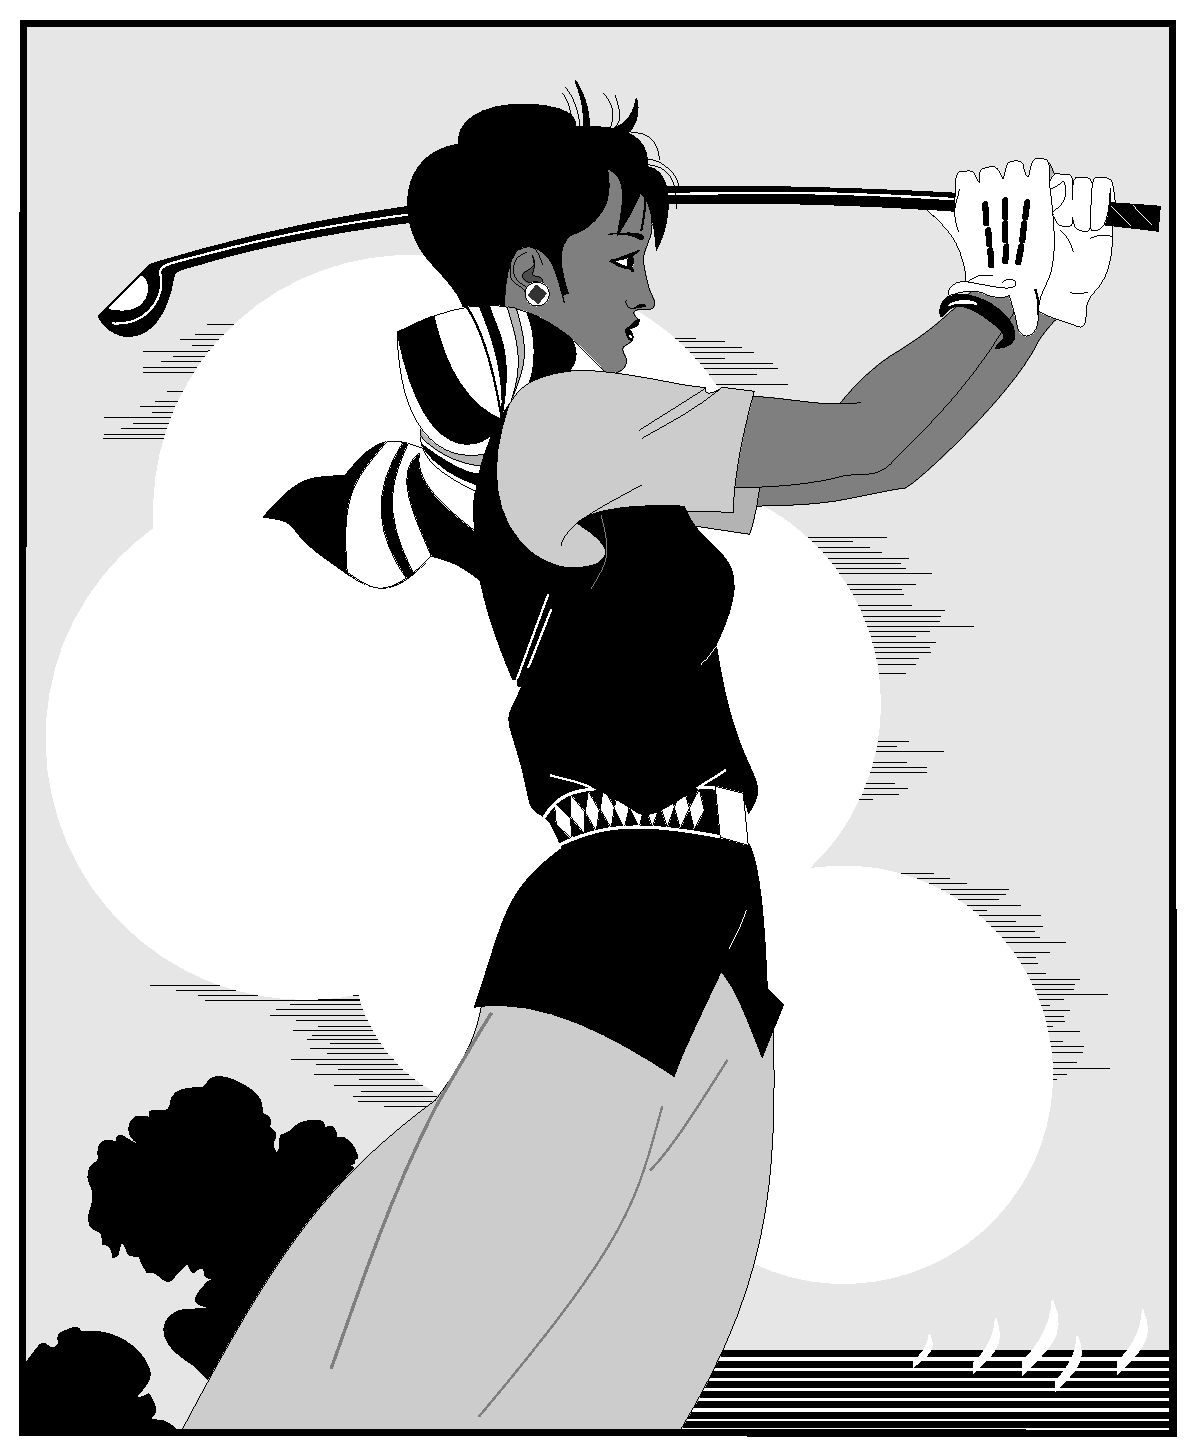
\includegraphics[width = 0.4\textwidth]{golfer}
	\bicaption[golfer1]{}{打高尔夫球的人}{Fig.$\!$}{The person playing golf}\vspace{-1em}
\end{figure}

其插入图片的代码及其说明如下。
\vspace{1em}\noindent\hrule
\begin{lstlisting}
\begin{figure}[htbp]
\centering
\includegraphics[width=0.4\textwidth]{文件名(.eps)}
\bicaption[标签名(英文)]{}{中文标题}{Fig.$\!$}
{English caption (首字母大写)}\vspace{-1em}
\end{figure}
\end{lstlisting}
\noindent\hrule
\begin{lstlisting}
figure环境的可选参数[htbp]表示浮动图形所放置的位置,h (here)表示当前位置,t (top)表示页芯顶部,b (bottom)表示页芯底部,p (page)表示单独一页。在word等软件中,图片通常插入到当前位置,如果当前页的剩余空间不够,图片将被移动到下一页,当前页就会出现很大的空白,其人工调整工作非常不便。由LaTeX提供的浮动图片功能,总是会按h->t->b->p的次序处理选项中的字母,自动调整图片的位置,大大减轻了工作量。
\centering命令将后续内容转换成每行皆居中的格式。
“\includegraphics”的可选参数用来设置图片插入文中的水平宽度,一般表示为正文宽度(\textwidth)的倍数。
\bicaption命令的使用需要调用ccaption宏包,它可以为图片或表格插入双语标题(博士学位论文要求),可选参数“标签名”为英文形式,一般不以图片或表格的数字顺序作为标签,而应包含一定的图片或表格信息,以便于文中引用(若图片、表格、公式、章节和参考文献等在文中出现的先后顺序发生了变化,其标注序号及其文中引用序号也会跟着发生变化,这一点是word等软件所不能做到的)。第4个参数中的“$\!$”表示-1/6个空铅宽度,这样可以缩小Fig.和Table与后面数字序号之间的水平距离。另外,图题或表题并不会因为分页而与图片或表格体分置于两页,章节等各级标题也不会置于某页的最底部,LaTeX系统会自动调整它们在正文中的位置,这也是word等软件所无法匹敌的。
注:硕士学位论文的图表只需要插入中文标题,因此需将\bicaption一句命令替换为如下两条命令(下同):
\caption{中文标题}
\label{标签名(英文)}
\vspace将产生一定高度的竖直空白,必选参数为负值表示将后续文字位置向上提升,参数值可自行调整。em为长度单位,相当于大写字母M的宽度。
引用方法:“见图~\ref{标签名(英文)}”、“如图~\ref{标签名(英文)}~所示”等。
\end{lstlisting}
\noindent\hrule\vspace{1em}
若需要将~2~张及以上的图片并排插入到一行中,则需要采用\verb|minipage|环境,如图~\ref{golfer2}~和图~\ref{golfer3}~所示。
\begin{figure}[htbp]
	\centering
	\begin{minipage}{0.4\textwidth}
		\centering
		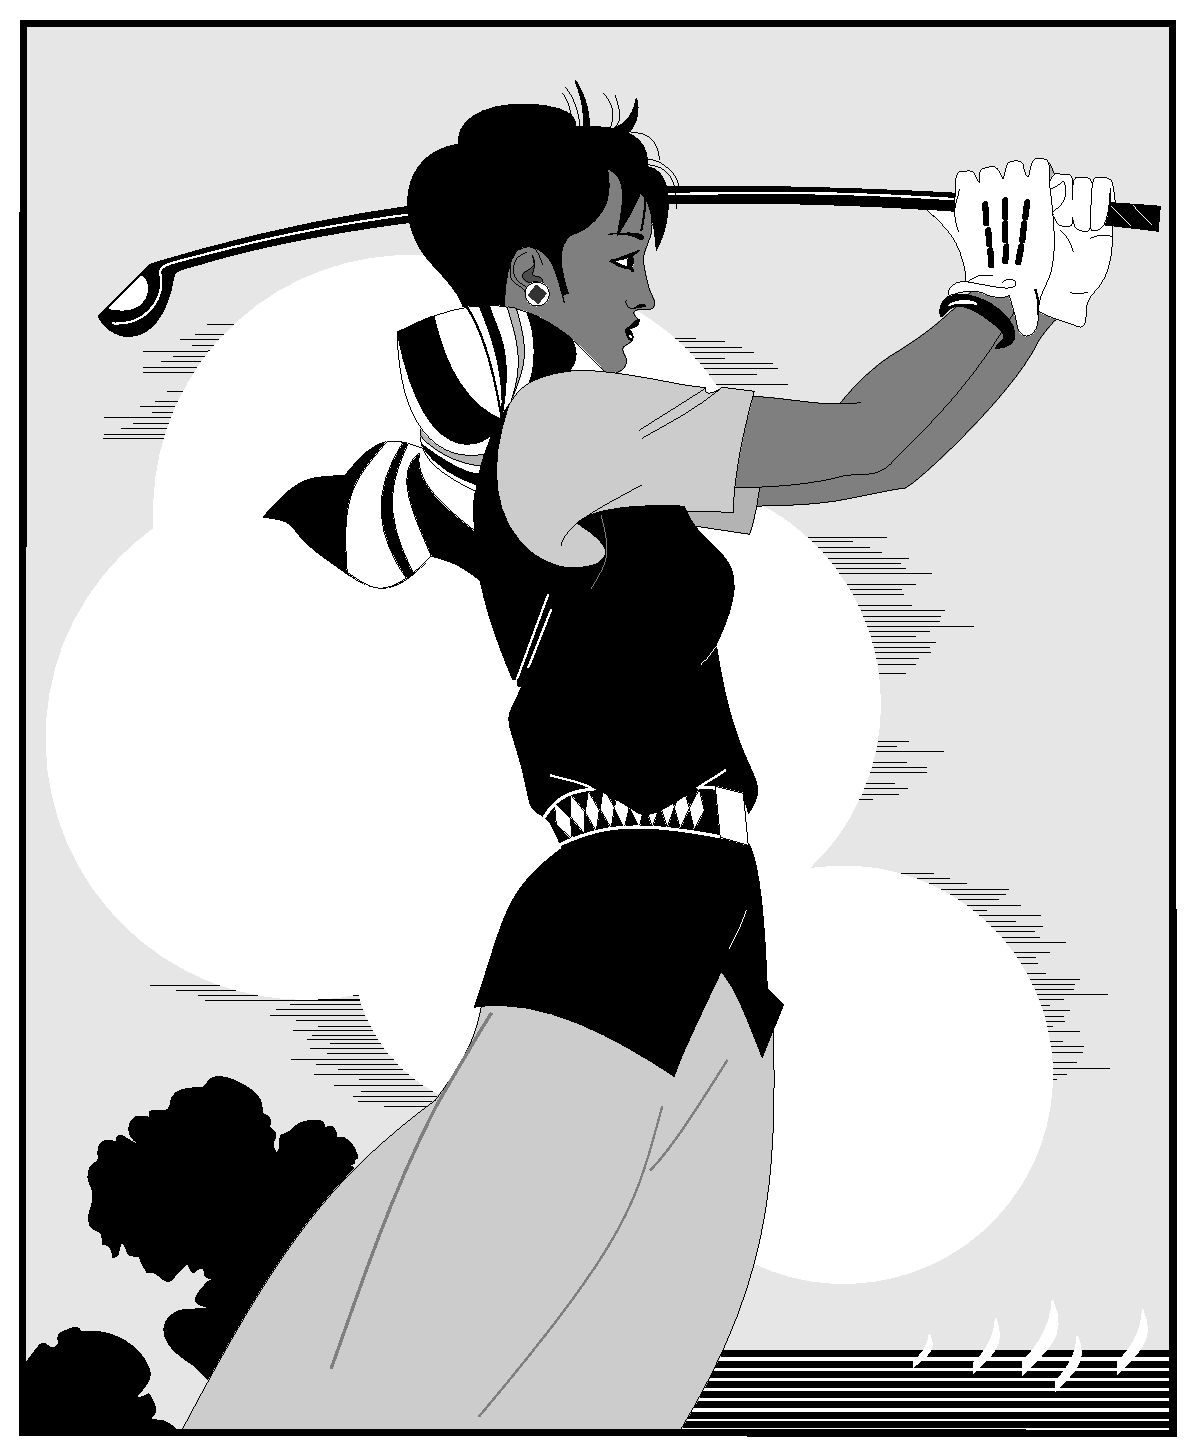
\includegraphics[width=\textwidth]{golfer}
		\bicaption[golfer2]{}{打高尔夫球的人}{Fig.$\!$}{The person playing golf}
	\end{minipage}
	\begin{minipage}{0.4\textwidth}
		\centering
		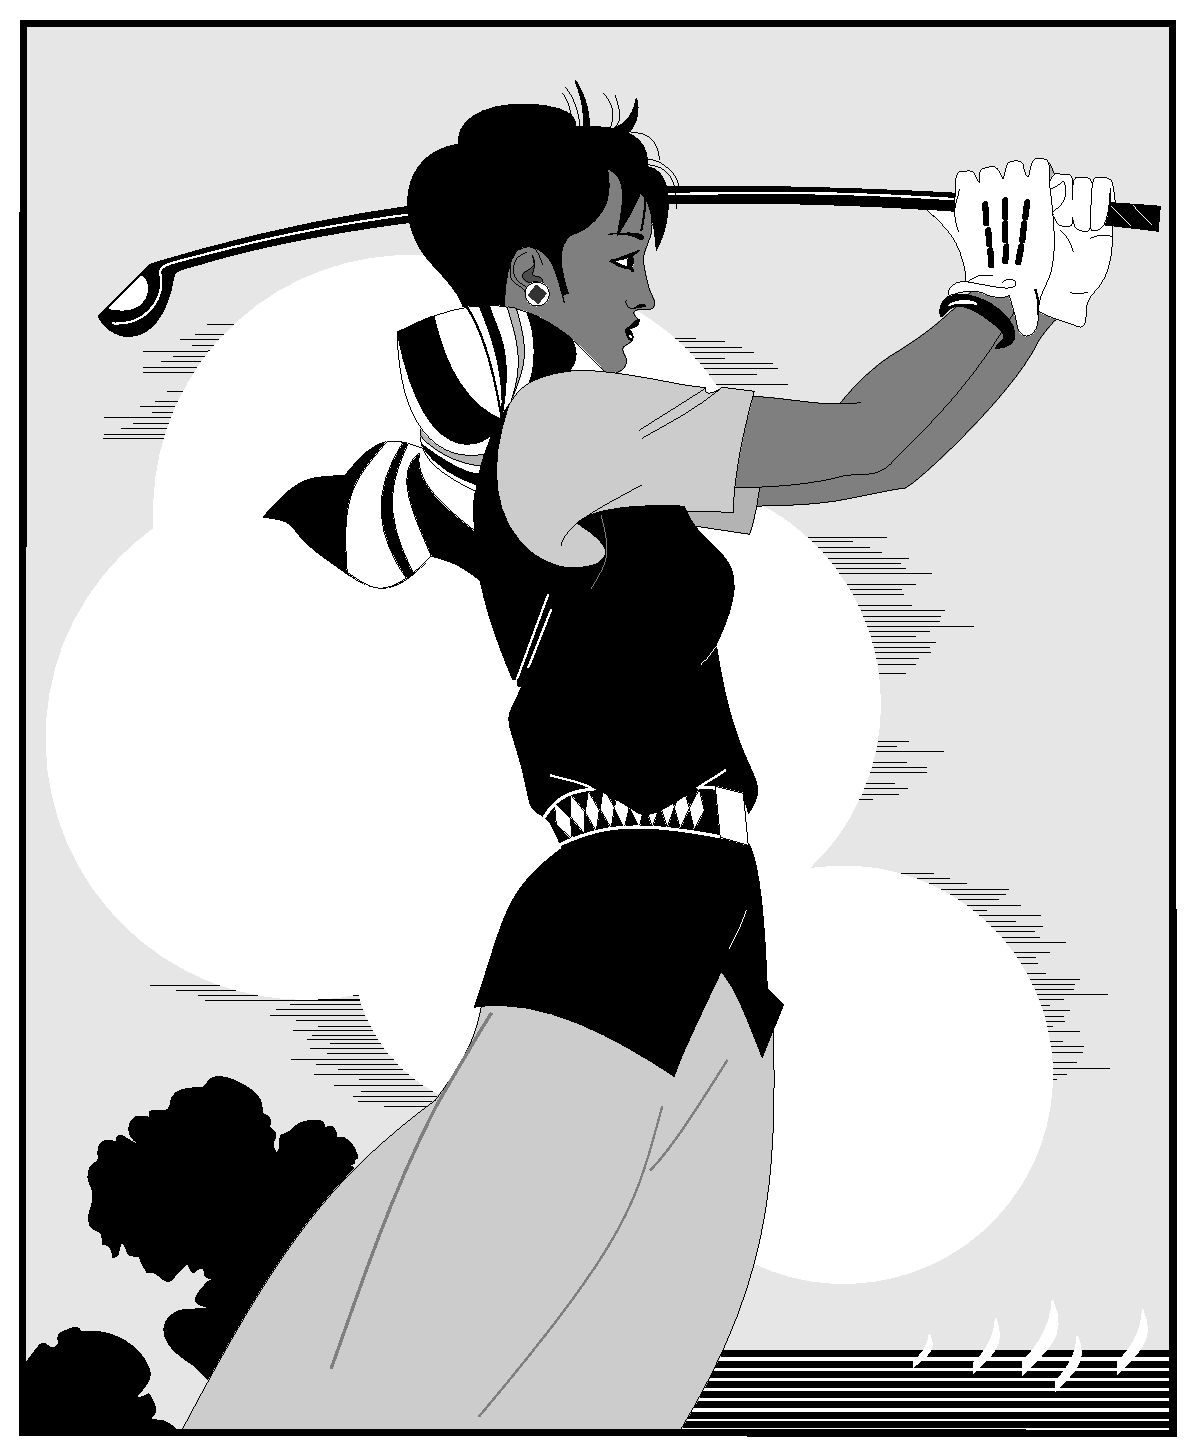
\includegraphics[width=\textwidth]{golfer}
		\bicaption[golfer3]{}{打高尔夫球的人}{Fig.$\!$}{The person playing golf}
	\end{minipage}\vspace{-1em}
\end{figure}

其代码如下所示。
\vspace{1em}\noindent\hrule
\begin{lstlisting}
\begin{figure}[htbp]
\centering
\begin{minipage}{0.4\textwidth}
\centering
\includegraphics[width=\textwidth]{文件名}
\bicaption[标签名]{}{中文标题}{Fig.$\!$}
{English caption}
\end{minipage}
\begin{minipage}{0.4\textwidth}
\centering
\includegraphics[width=\textwidth]{文件名}
\bicaption[标签名]{}{中文标题}{Fig.$\!$}
{English caption}
\end{minipage}\vspace{-1em}
\end{figure}
\end{lstlisting}
\noindent\hrule
\begin{lstlisting}
minipage环境的必选参数用来设置小页的宽度,若需要在一行中插入n个等宽图片,则每个小页的宽度应略小于(1/n)\textwidth。
\end{lstlisting}
\noindent\hrule

\BiSection{具有子图的图片插入方法}{The method of inserting figures with subfigures}

图中若含有子图时,需要调用~subfigure~宏包。博士学位论文规范要求不止总图的标题为中英文形式,其各个子图也应具有中英文形式的标题。
然而~ccaption~宏包却无法实现子图的中英文标题功能,这里采用对\verb|\subfigure|命令进行嵌套的方法来实现子图的中英文标题功能,如图~\ref{golfer4}~所示。

\begin{figure}[htbp]
	\centering
	\subfigure{\label{golfer41}}\addtocounter{subfigure}{-2}
	\subfigure[The person playing golf]{\subfigure[打高尔夫球的人~1]{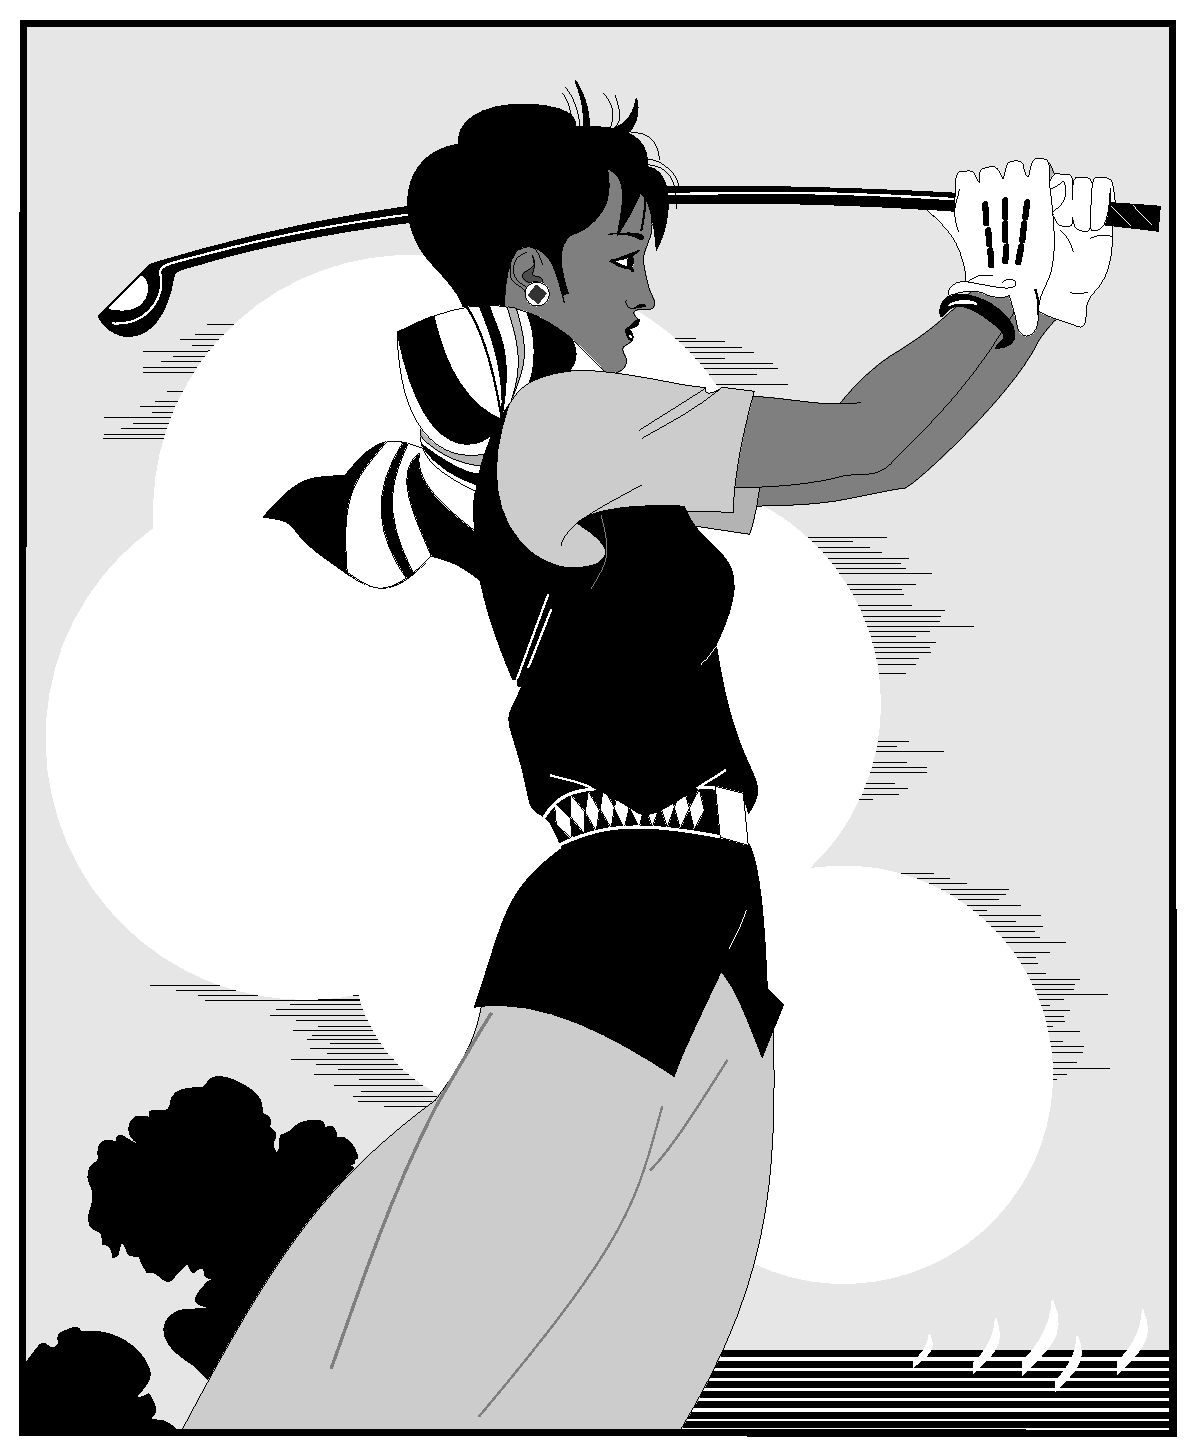
\includegraphics[width=0.4\textwidth]{golfer}}}
	\subfigure{\label{golfer42}}\addtocounter{subfigure}{-2}
	\subfigure[The person playing golf]{\subfigure[打高尔夫球的人~2]{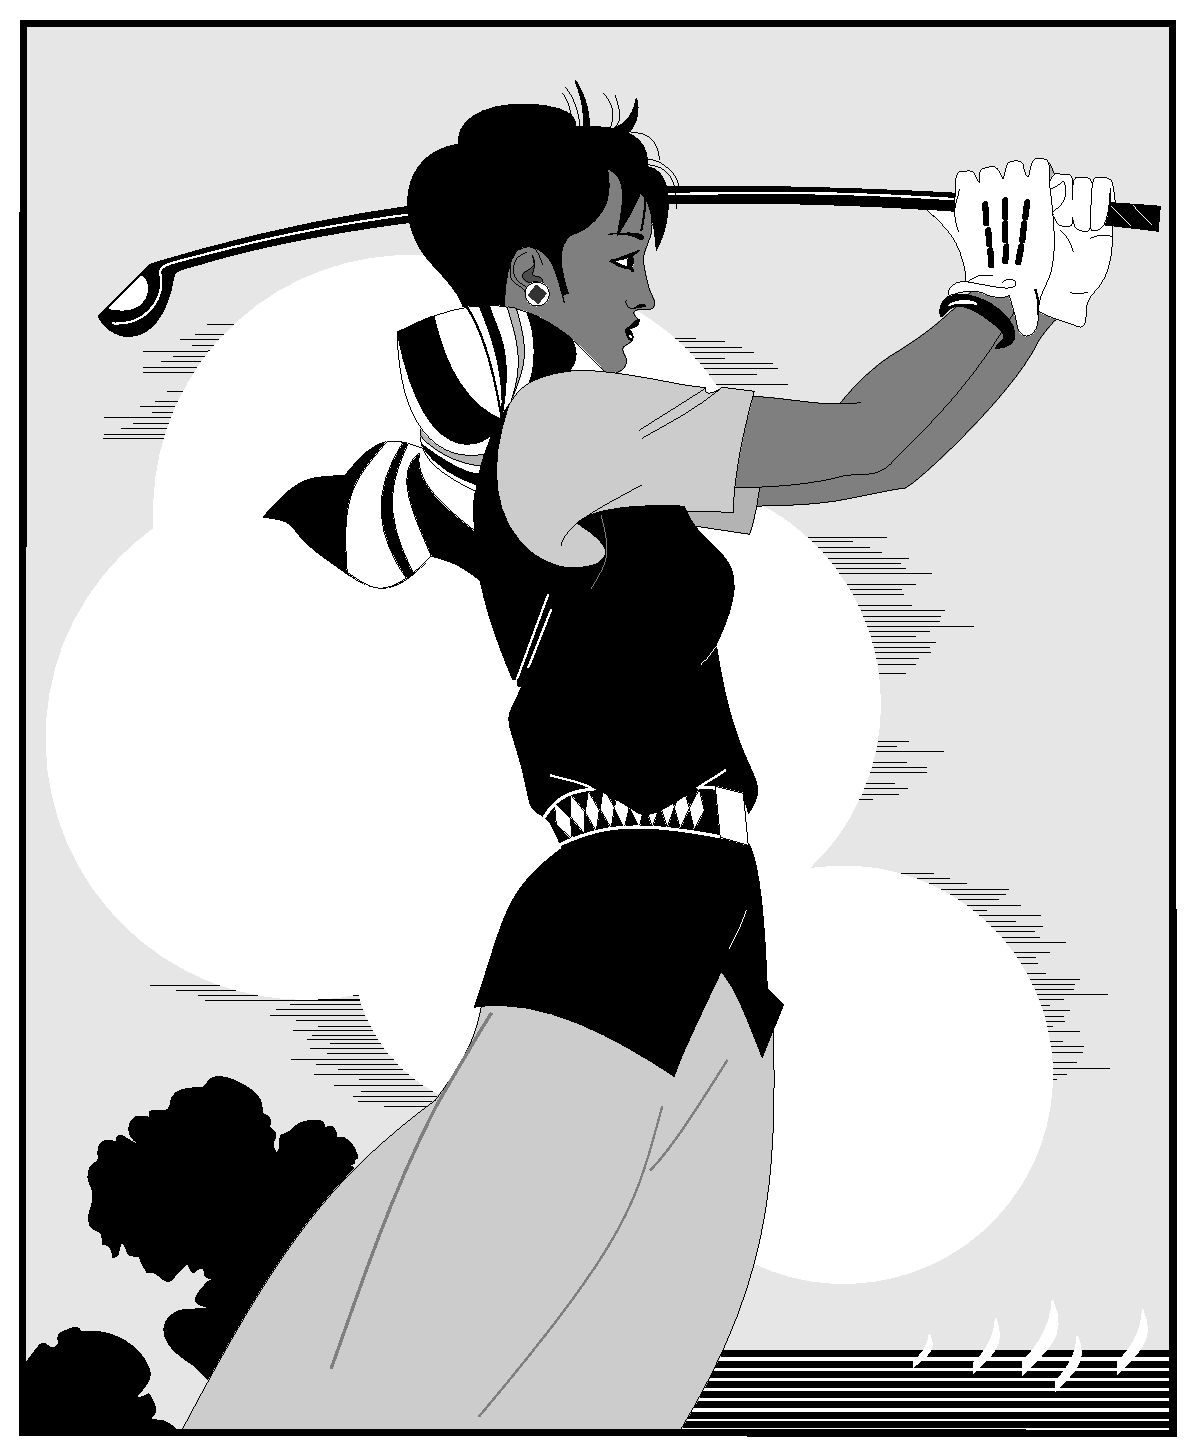
\includegraphics[width=0.4\textwidth]{golfer}}}
	\bicaption[golfer4]{}{打高尔夫球的人}{Fig.$\!$}{The person playing golf}\vspace{-1em}
\end{figure}

其代码及其说明如下。
\vspace{1em}\noindent\hrule
\begin{lstlisting}
\begin{figure}[htbp]
\centering
\subfigure{\label{第1个子图标签名}}\addtocounter{subfigure}{-2}
\subfigure[The 1st subfigure caption]{\subfigure[第1个子图标题]
{\includegraphics[width=0.4\textwidth]{文件名}}}
\subfigure{\label{第2个子图标签名}}\addtocounter{subfigure}{-2}
\subfigure[The 2nd subfigure caption]{\subfigure[第2个子图标题]
{\includegraphics[width=0.4\textwidth]{文件名}}}
\bicaption[总标签名]{}{中文总标题}{Fig.$\!$}{The total caption}
\vspace{-1em}
\end{figure}
\end{lstlisting}
\noindent\hrule
\begin{lstlisting}
\addtocounter把指定的值加到计数器上,这里是对subfigure计数器进行减2操作。这是因为每插入1个子图,就调用3次\subfigure命令,第1次调用\subfigure命令用来生成紧随其后所插入子图的标签,而之后的双层嵌套调用\subfigure命令用来插入子图并生成该子图的中英文标题。因此,每插入1张子图,subfigure计数器的值就自动加3,为了使得子图的序号能每次加1,则需在每插入1张子图前手动把subfigure计数器的值减2。
\subfigure命令的双层嵌套使用可用来生成中英文标题,其内层\subfigure命令用来插入子图并生成中文标题,外层\subfigure命令将插入的子图和中文标题作为一个整体,生成这个整体的英文标题,因此英文标题会置于中文标题的下面。
硕士学位论文只需要中文标题,其代码如下:
\begin{figure}[htbp]
\centering
\subfigure[第1个子图标题\label{第1个子图标签名}]
{\includegraphics[width=0.4\textwidth]{文件名}}
\subfigure[第2个子图标题\label{第2个子图标签名}]
{\includegraphics[width=0.4\textwidth]{文件名}}
\caption{中文总标题}\label{总标签名}
\vspace{-1em}
\end{figure}
引用方法:总图的引用方法同本章第1节,子图的引用方法用\ref{第n个子图标签名}来代替。
\end{lstlisting}
\noindent\hrule\vspace{1em}

子图的引用示例:如图~\ref{golfer41}~和图~\ref{golfer42}~所示。

若想获得插图方法的更多信息,请参见网络上的~\href{ftp://ftp.tex.ac.uk/tex-archive/info/epslatex.pdf}{Using Imported Graphics in \LaTeX and pdf\LaTeX}~文档。 
